\documentclass[openany]{book}

\input{../../../latex_preambule_style/preambule}
\input{../../../latex_preambule_style/styleCoursCycle4}
\input{../../../latex_preambule_style/styleExercices}
\input{../../../latex_preambule_style/styleExercicesAideCompetences}
%\input{../../latex_preambule_style/styleCahier}
\input{../../../latex_preambule_style/bas_de_page_cycle4}
\input{../../../latex_preambule_style/algobox}


%%%%%%%%%%%%%%%  Affichage ou impression  %%%%%%%%%%%%%%%%%%
\newcommand{\impress}[2]{
\ifthenelse{\equal{#1}{1}}  %   1 imprime / affiche sur livre  -----    0 affiche sur cahier 
{%condition vraieé
#2
}% fin condition vraie
{%condition fausse
}% fin condition fausse
} % fin de la procédure
%%%%%%%%%%%%%%%  Affichage ou impression  %%%%%%%%%%%%%%%%%%
 \usepackage{geometry}
 \geometry{top=1.5cm, bottom=0cm, left=2cm , right=2cm}
%%%%%%%%%%%%%%%%%%%%%%%%%%%%%%%%%%%%%%%%%%%%%%%%

\begin{document}

\begin{dtl}[Solides de l'espace]

\begin{description}
\item[$\square$] 
(Se) repérer sur une droite graduée, dans le
plan muni d’un repère orthogonal, dans un
parallélépipède rectangle ou sur une sphère.
\item[$\triangleright$] Abscisse, ordonnée, altitude.
\end{description}
\end{dtl}

\Exe


On donne le dessin d'une maison dont la base est un rectangle.

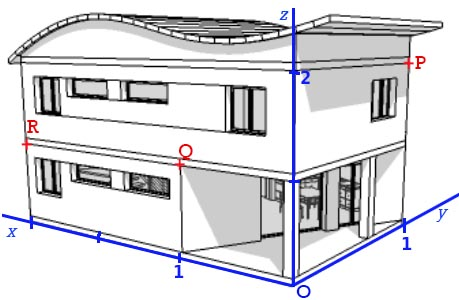
\includegraphics[scale=0.5]{RepE-21.jpg} 

\begin{enumerate}
\item Déterminer les coordonnées des points $P$, $Q$ et $R$.
\item Quelles sont les coordonnées du point $S$ qui se trouve à la même hauteur que $P$ est sur l'arête cachée de la maison.
\end{enumerate}


\Exe


La somme des points des faces opposées d'un dé est égale à 7. Détermine les coordonnées de tous les points de chaque face.

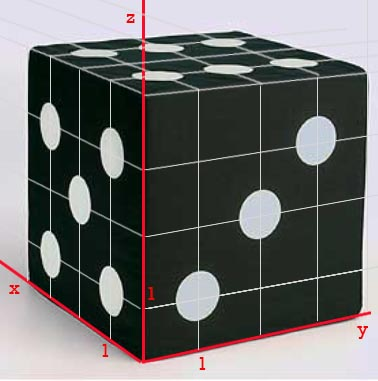
\includegraphics[scale=0.5]{RepE-22.jpg} 


\Exe

Pour réaliser un tas de sable, Albert creuse un fossé dont les parois sont verticales et dont la base est délimitée par deux cercles dont l’un a un rayon double de l’autre.

Avec tout le sable extrait il forme au milieu un cône de révolution dont la base coïncide parfaitement avec le disque autour duquel il a creusé.

\begin{minipage}{0.68\linewidth}
\begin{enumerate}
\item On sait que la profondeur du fossé est de 15 cm et que le grand cercle a pour rayon 2 m. Quel est le volume de sable qu’Albert a déplacé?
\item Quelle est la hauteur du tas de sable? 
\end{enumerate}
\end{minipage}
\hfill
\begin{minipage}{0.30\linewidth}
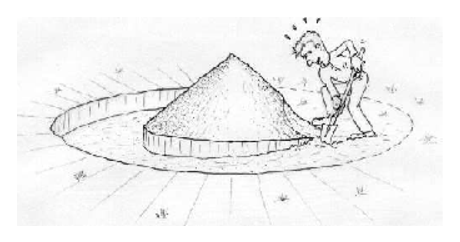
\includegraphics[scale=0.6]{DTL.eps} 
\end{minipage}

\end{document}